\documentclass[a4paper,french,bookmarks]{article}

\usepackage{./Structure/4PE18TEXTB}

\usepackage{graphicx}
\usepackage{listings}

% Définir les couleurs pour les mots clés
\definecolor{keywords}{RGB}{255,0,90}

% Définir les mots clés
\lstset{
    language=C,
    keywordstyle=\color{keywords}\bfseries,
    morekeywords={Données,graphe,deja_vu,G,listes,adjacences,sommet,départ,s,a_traiter,implémentée,file,deja_vu,dist,pred,tant,faire,retourner,pour,tout,voisin,tel,que,est}
}


\newboxans
\usepackage{booktabs}

\begin{document}

    \renewcommand{\thesection}{\Roman{section}} 
    \renewcommand{\thesubsection}{\thesection.\Alph{subsection}}
    \setlist[enumerate]{font=\color{white5!60!black}\bfseries\sffamily}
    \renewcommand{\labelenumi}{\thesection.\arabic{enumi}.}
    \renewcommand*{\labelenumii}{\alph{enumii}.}
    \renewcommand*{\labelenumiii}{\alph{enumiii}.}
    
    \def\authorvar{DRISSI Rayan}
    \stylizeDocSpe{Info}{Chapitre 4}{}{Algoritme des graphes}

    \section{Rappel}

    
    \begin{definition}{Graphe Orienté}{}
        Un graphe orienté est un couple $G = (S, A)$
        
        \begin{enumerate}
            \itt $S$ est un ensemble de sommets;
            \itt $A \subseteq S \times S$ est un ensemble d'arcs 
        \end{enumerate}
        Usuellement, on représente les arcs d'un graphe par des flèches entre les sommets 
    \end{definition}
    
    \begin{definition}{Adjacence}{}
        Soit $G = (S, A)$ un graphe orienté. 
        Si $(x,y) \in A $
        \begin{enumerate}
            \itt On note ainsi $x \to y $ plutôt que $(x,y) \in A$
            
            \itt On dis que $y$ est un successeur de x (ou voisin de x)
            
            \itt On dit que x est un prédécesseur de y
            
            \itt Si $x=y$, on dis que l'arc $(x,x)$ est une boucle 
        

        \end{enumerate}
    
    \end{definition}
    
    \begin{definition}{Chemin}
        Soit $G = (S, A)$ un graphe orienté,
        Soit $(u,v) \in S^2$
        
        Un chemin de u à v est une sequence $x_0 \dots x_n$ sommets de S tq:
        \begin{enumerate}
            \itt $x_0 = u$
            \itt $x_n = v$
            \itt $x_i \to x_{i+1} \forall i \in \llbracket 0, n+1 \rrbracket$
        \end{enumerate}
        
    \end{definition}
    
    \begin{definition}{Arbre, Fôrets}{}
        
        Un graphe non orienté connexte actclique est appeler un arbre 
        Un ensemble d'arbres est appelé une foret
    
    \end{definition}

    \begin{theorem}{}{}
        Si $G = (S,A) $ est un ensemble avec $|S| = n$, alors $|A| = n-1$
    \end{theorem}
    
    
    
    \begin{form}{Complexité}{}
        \begin{enumerate}
            \itt Tester si u \to v se fait en $\bcO(n)$
            
            \itt Parcourir les voisins de $s\in S$ se fait en $\bcO(n)$
        \end{enumerate}
    \end{form}
    
    
    \begin{definition}{Liste d'adjance}{}
        Soit $G = (S,A)$ un graphe avec $S = \llbracket 0, n-1 \rrbracket$
    \end{definition}
    \begin{form}{Implementation}{}
        \begin{enumerate}
            \itt En OCaml, on utilise une variable de type \camlline{(int list) array}
            
            \itt En C on peut par exemple:
                \begin{enumerate}
                    
                    \itt Avoir un tableau tq g[s] pointe vers le début d'une liste chainée;
                    
                    \itt Avoir un tab tq g[s] pointe vers le debut d'un tableau de taille $d_t(S)$
                    contenant les voisins 
                \end{enumerate}
        \end{enumerate}
    \end{form}
    \begin{form}{Complexité}{}
        \begin{enumerate}
            
            \itt Tester si u \to v se fait en $\bcO(d_t(u))$
            
            \itt Parcourir les voisins de $s \in S$ se fait en $\bcO(d_t(s))$
        \end{enumerate}
    \end{form}

    \begin{definition}{Graphe Pondérés}{}
        En pratique, on utilisera le type float pour les poids
        Pour la representation par matrice d'adjance, on choisit la variante suivante:
        %
        \[ M_{i,j} = \left\lbrace\begin{array}{rl}
            \omega\p{i \to j} &\text{si } i \to j \\
            0 &\text{si } i = j\\
            +\infty &\text{sinon}
        \end{array}\right. \]
    
    \end{definition}


    \begin{definition}{Parcours en Largeur BFS}{}
    
        Dans un graphe non pondéré $G = (S,A)$ voici le parcours en largeur 
        
        Cet algorithme parcourt tous les noeuds d'un graphe en commençant par le noeud initial et en explorant d'abord les voisins directs avant de continuer avec les voisins des voisins. La file (queue) est utilisée pour stocker les noeuds à explorer dans l'ordre où ils ont été découverts.
        
        \\
        
        
        
        \begin{lstlisting}
Algorithme 1 : Parcours en largeur, calcul des distances
Données : Un graphe G donné par listes d'adjacences, un sommet de départ s
a_traiter ← {s} ; // implémentée par une file
deja_vu ← [Faux, . . . , Faux] ;
dist ← [−1,...,−1]; pred ← [−1,...,−1]; deja_vu[s] ← Vrai ; dist[s] ← 0 ;
pred[s] ← s ;
tant que a_traiter est non vide faire
    u ← sortir le prochain élément de a_traiter ;
    pour tout voisin v de u tel que deja_vu[v] est Faux faire
        a_traiter ← a_traiter ∪ {v} ; deja_vu[v] ← Vrai ;
        dist[v] ← dist[u] + 1 ;
        pred[v] ← u ;
    retourner dist, pred ;
        \end{lstlisting}
        
        


    \end{definition}



    
    \begin{lemma}{}{}
        $\forall d \in \bcN$ on a $ P(d)$ suivante:
        
        $P(d) $: Les sommet a distance $d$ de $s$ sont inséré dans la file avant tous ceux a distance
        $\geqslant d+1 $ de s 
    \end{lemma}
    \begin{nproof}{}{}
        A rediger
        
    \end{nproof}
    
    \begin{theorem}{Correction}{}
        A la fin de l'algo ça renvoie bien le bon resultat  
    \end{theorem}
    \begin{nproof}
        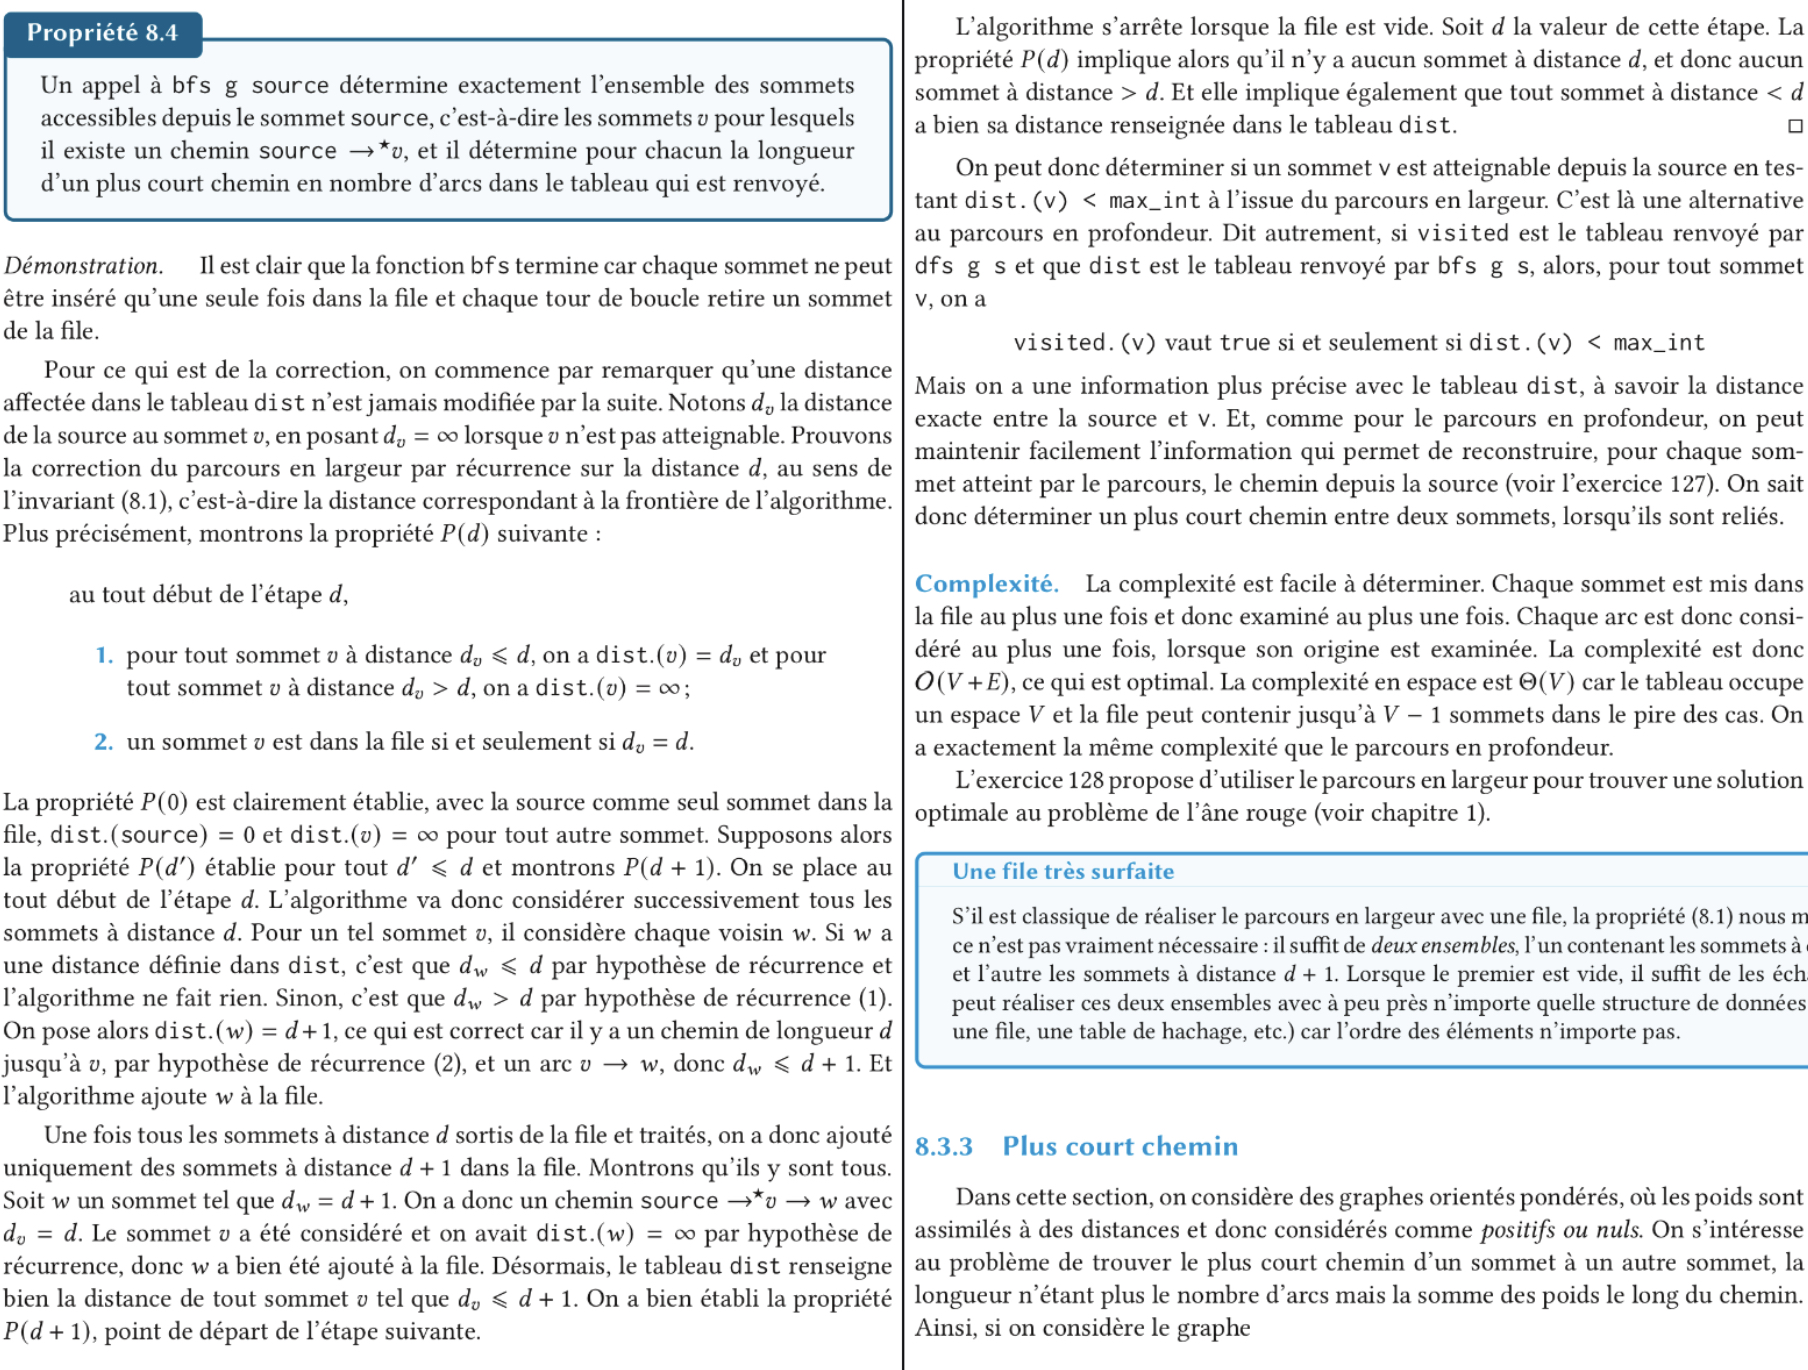
\includegraphics[scale=0.5]{MPI - Informatique/Cours/Dessin/ProofBFS.jpeg}
    \end{nproof}
    
    \section{Dijkstra }
    
    L'algoritme de Dijktra permet de trouver le plus cours chemin en poids entre deux sommet  

    \begin{definition}{Heuristique}{}
        Soit $G = (S,A,\omega)$ un graphe ponderé
        
        Une \textbf{heuristique} est une fonction $S \times S \to \bcR^*$ tq h(u,t) donne une approxiamtion de $\sigma(u,t)$ 
        On impose également que $h(u,v) = 0$   $\forall u\in S$
    \end{definition}
    \begin{example}{}{}
        Si G est le graphe du reseau routier européen
        \begin{enumerate}
            \itt $h(u,t)$ distance a vol d'oiseau || $||_2$
    
            \itt $h(u,t)$ distance manhantan
            
            
        \end{enumerate}
    \end{example}
    
    \begin{definition}{Heuristique admisible | Monotone}{}
        Soit $G = (S,A,\omega) $ un graphe pondéré
        Soit h une heuristique 
        \\
        
         h est dite \underline{admisible} si: \[  \forall (v,t) \in S^2 \quad h(v,t) \geqslant \delta(v,t) \]
        Autrement dis si on ne fais jamais de suraproxiamtion
        
        \\
        h est dite \underline{monotone} si: \[ \forall t \in S,\quad \forall u \to v \in A \text{\quad  \quad On a:  }\quad \quad h(u,t) \geqslant \omega + h(u,v) \]
    \end{definition}
    
    
    
    \begin{property}{Complexité/Terminaison}{}
        L'algo $A^*$ termine en temps polynomial 
    \end{property}
    \begin{nproof}{}{}
        A rediger 
    \end{nproof}
    \begin{corollary}{}{}
        Dijkstra est correct 
    \end{corollary}
    
    \begin{definition}{}{}
        
    \end{definition}

\end{document}
 